The surge in energy consumption levels is inevitable for modern societies. Their sustainability depends on it. The \usebibentry{EIA2017}{title} report \citeyearpar{EIA2017} published by the \usebibentry{EIA2017}{institution} projects a 28\% increase in world energy consumption between 2015 and 2040, assuming continuous improvement in known technologies based on current trends. As shown in Figure \ref{cht:energySources}, the consumption of ``petroleum and other liquid fuels" alone will grow by 18\%, which will account for 31\% of total world energy consumption in 2040.

\begin{figure}[b!]
    \centering
    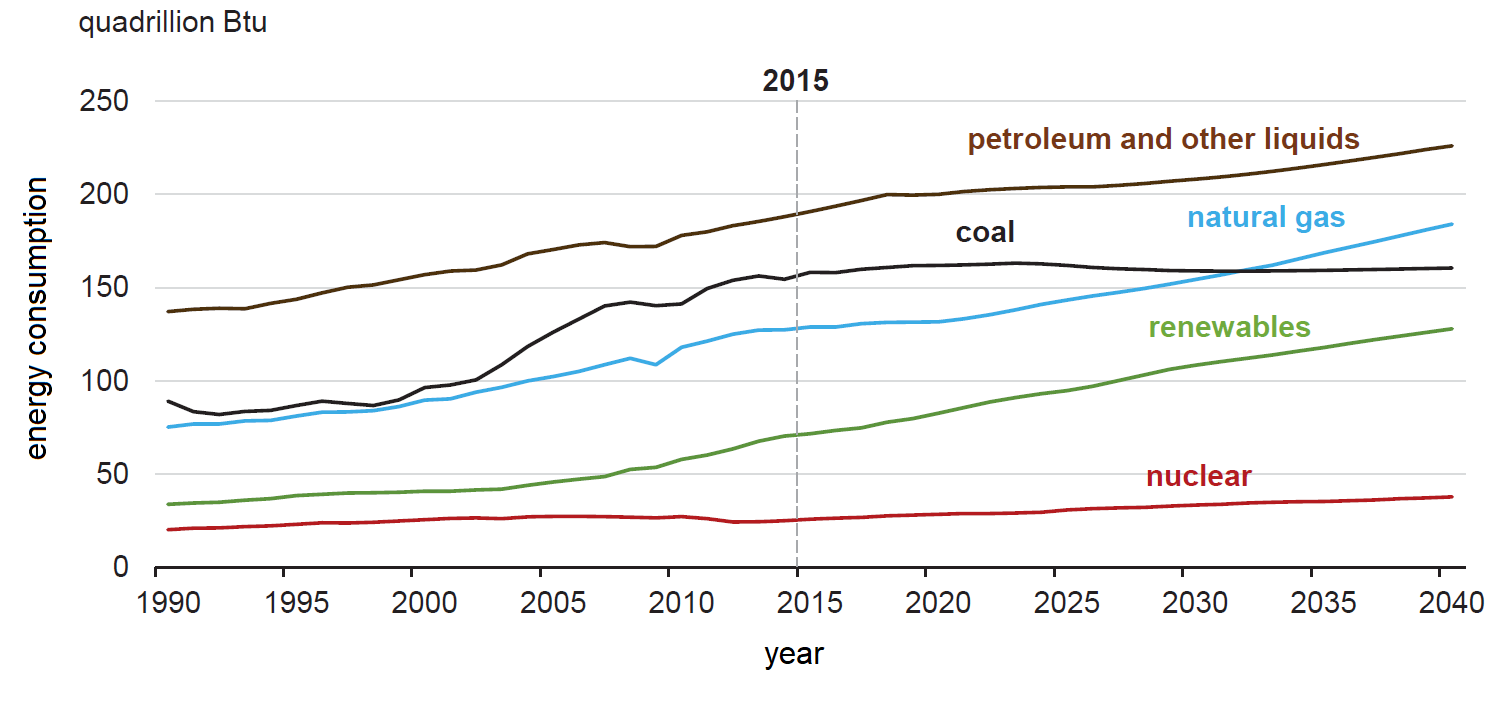
\includegraphics[width=\textwidth]{img/chart/chtEiaEnergy}
    \caption{World energy consumption by energy source \citep{EIA2017}}
    \label{cht:energySources}
\end{figure}

It is becoming more and more challenging to meet the ever-increasing demand for petroleum. Most of the existing major oilfields are already at a mature stage and the number of new significant discoveries per year is decreasing. Therefore, at this point in time, it is crucial to focus on methods of improving petroleum production from existing reservoirs. A big subset of such methods fall under the category of Enhanced Oil Recovery (EOR).

Challenges and technology gaps within EOR, \index{EOR!challenges} which need to be addressed in the coming research programs, have been identified in the OG21 strategy document on ``Exploration and Increased Recovery" \citep{OG21}: In particular, there is a need for more cost-efficient EOR chemicals, and to assure environmentally acceptable methods to avoid unwanted discharge to sea. Improved petroleum resource exploitation by EOR has also been given special attention in a report on increased recovery in the Norwegian Continental Shelf by the Norwegian Department of Oil and Energy \citep{Am2010}. There is therefore a clear need for increased competence in new technologies in the field of EOR. 

There has recently been an increasing interest in applying nanotechnology to EOR but still many topics are uncovered. Nanotechnology, \index{Nanotechnology} which has mainly been developed in mechanical engineering, medicine and biological sciences, is expected to have a large potential for EOR applications. This technology has a wide range of applications relevant to EOR, from employing general concepts and principles of nanotechnology, to advanced reservoir monitoring using nano-sensors and nano-analysis, to more specific technologies which make up for the shortcomings in traditional EOR methods \citep{Fletcher2010, Ayatollahi2012, Cocuzza2011}. The latter includes tailoring chemical molecules for more efficient EOR, as well as smart and more effective delivery of EOR agents. Such technologies as efficient drug delivery in the human body may be applied to improve efficiency in chemical flooding.

This PhD work is part of the HyGreGel\index{HyGreGel|(} (Hybrid Green nano-Gels) project. The HyGreGel project addresses the need for more efficient water diversion techniques by improved in-depth placement of gelling chemicals to increase waterflood recovery and reduce unwanted water circulation in heterogeneous reservoirs. The project recognizes the environmental challenges using chemicals and emphasizes the development of green chemical systems for such applications.